\subsection{Curricular weighting}\label{subsec:curricular_weighting}


\citet{curricular_weighting_2024} propose \curricularWeighting, 
which is a weighting scheme for the negative samples 
in the context of \ac{cl}, which emulates human learning \citet{curriculum_wang_2022,curriculum_HGNNs_2024}.
Initially, the model is trained on easy negative samples and gradually prioritizes harder negative samples 
as displayed in \autoref{fig:curriculum_learning_samples}. %\citet{curricular_weighting_2024,curriculum_Soviany_2022}.
Therefore, the weight of hard negative samples is increased over time according to the model performance.
Furthermore, the authors introduce a $\mathcal{L}_2$ regularization term to mitigate the influence of \acp{fn}.

\begin{figure}[!htb] % h = here, t = top, b = bottom, p = page of floats
    \centering
    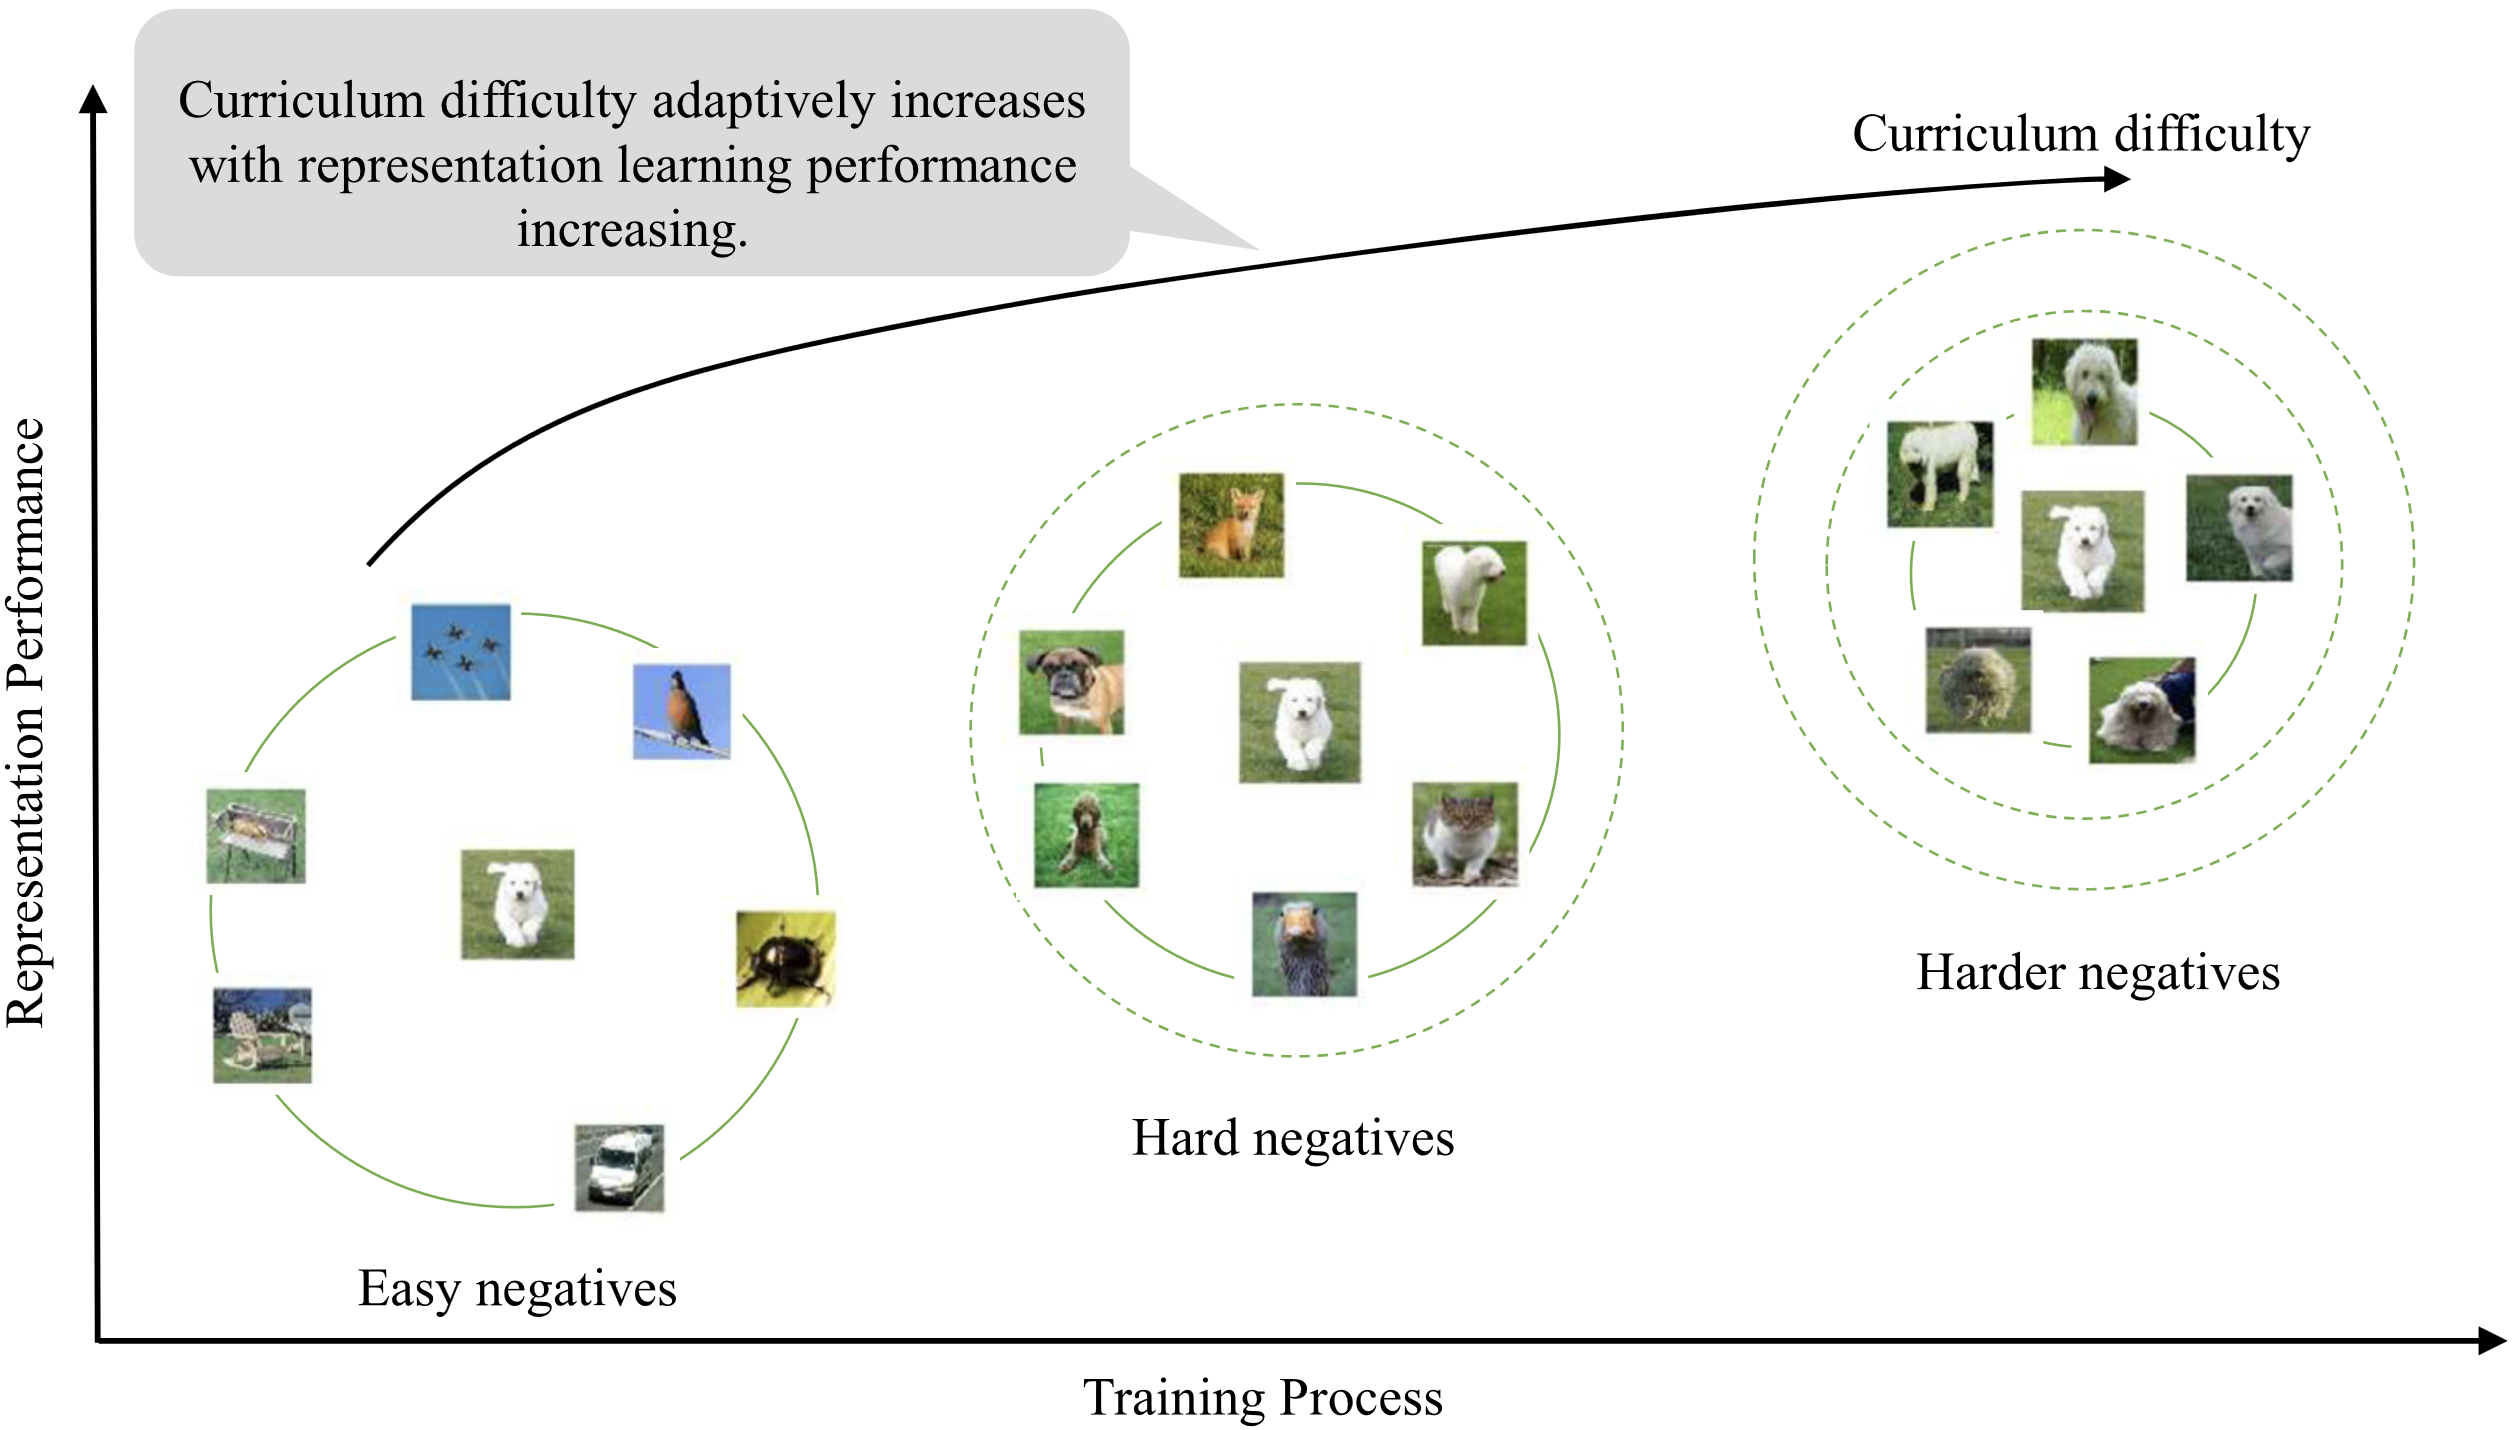
\includegraphics[width=360pt]{images/curriculum_learning_samples.png}
    \caption{Selection of negative samples for different stages of the training process 
    from \citet{curricular_weighting_2024}.
    Initially, the model is trained on easy negative samples.
    The difficulty of the negative samples is gradually increased over time.
    Solid circles represent the samples that are prioritized for training.
    }
    \label{fig:curriculum_learning_samples}
\end{figure}

% This approach considers samples from the same batch that are harder to distinguish from the anchor 
% than its positive sample obtained by an augmentation, hard negatives.
Firstly, the embeddings are $\mathcal{L}_2$ normalized.
Secondly, the similarity between the anchor and the other samples in the batch is calculated via the dot product.
The similarity of the positive pair is denoted $s_{ii'}$ while the similarity of the negative pair is designated $s_{ij}$.
If the similarity of a negative pair is bigger than the similarity of the positive pair, 
i.e. $s_{ij} > s_{ii'}$, the negative pair is considered a hard negative and 
the weight of the negative sample is multiplied by a factor $w_{ij}$ 
as illustrated in \Eqref{eq:curricular_negative_weighting}.

\begin{equation}
    N(i,j,t) = \left\{\begin{array}{ll} s_{ij}, & s_{ij} \le s_{ii'} \\
        s_{ij} \cdot  w_{ij}, & s_{ij} > s_{ii'}\end{array}\right. ,\text{ where }w_{ij} = t + s_{ij}
    \label{eq:curricular_negative_weighting}
\end{equation}

$w_{ij}$ is governed by the negative pair's similarity $s_{ij}$ emphasising hard negatives 
and the parameter $t$ which is adapted during training.
At the beginning of the training process, $t$ is set close to zero and thus, $w_{ij} < 1$ 
to assign smaller relative weights to hard negatives.
As the training progresses, $t$ is increased to assign higher weights $w_{ij} > 1$ to hard negatives.

\begin{equation}
    r_i(j) = \frac{\left| \frac{\partial \mathcal{L}_i}{\partial s_{ij}} \right|}
    {\left| \frac{\partial \mathcal{L}_i}{\partial s_{ii'}} \right|}
    \label{eq:curricular_weighting_ratio}
\end{equation}


By calculating the ratio $r_i(j)$ of the hard negative gradient and positive gradient 
with respect to the loss for different values of $t$ by \Eqref{eq:curricular_weighting_ratio}, 
the authors show that the model gradually focuses on hard negatives.
The resulting plot is depicted in \autoref{fig:gradient_ratio_hard_neg_pos}.

\begin{figure}[!htb] % h = here, t = top, b = bottom, p = page of floats
    \centering
    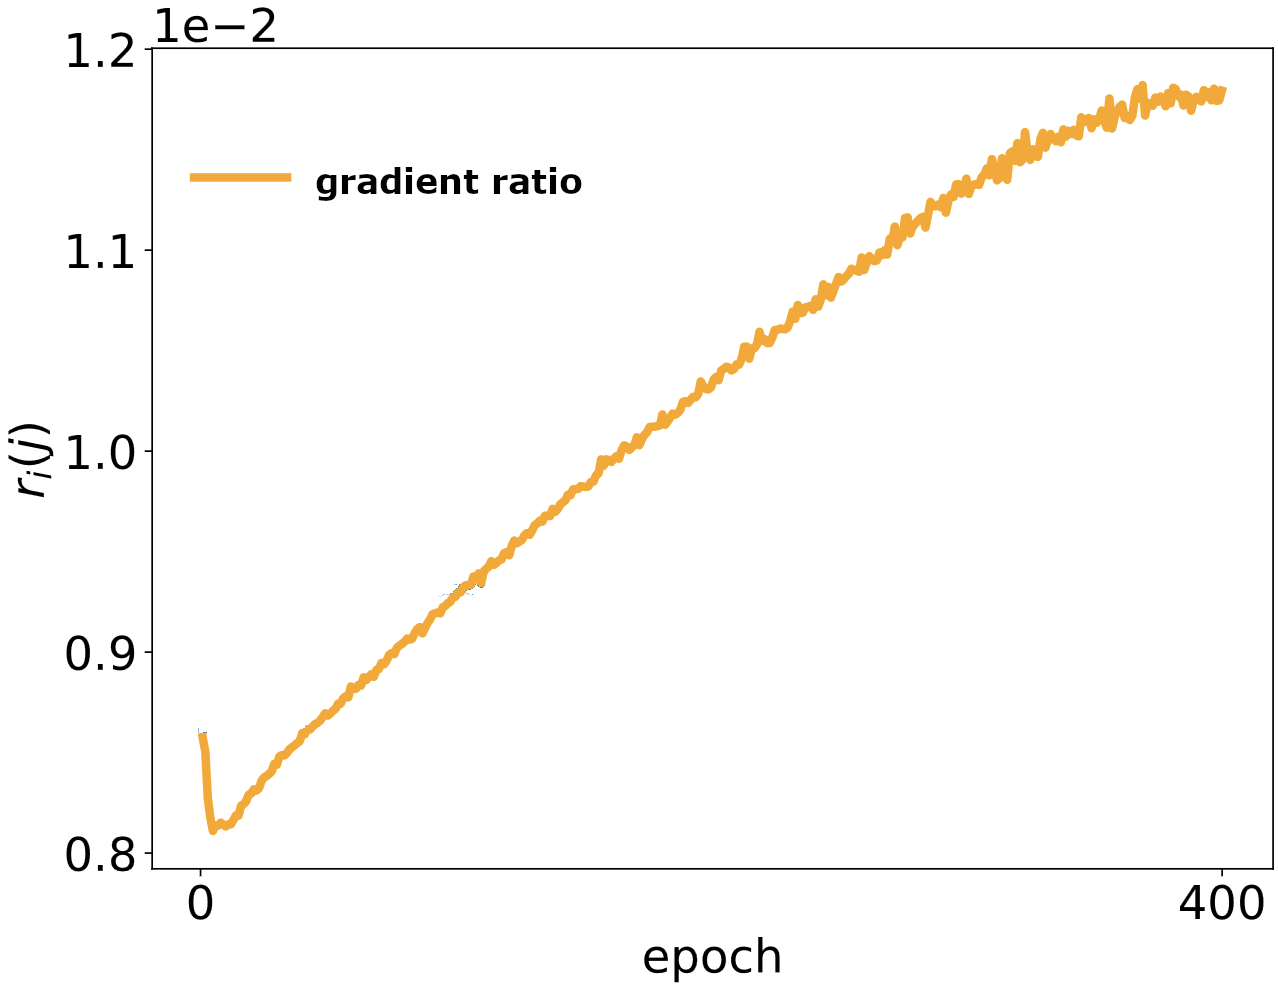
\includegraphics[width=280pt]{images/ratio_hard_neg_pos_gradients_only_ratio.png}
    \caption{Display of the gradient ratio of hard negative and positive samples throughout training 
    similar to \citet{curricular_weighting_2024}.
    As the training progresses, the model focuses more on hard negative samples, i.e. the ratio increases.
    }
    \label{fig:gradient_ratio_hard_neg_pos}
\end{figure}

The parameter $t$ is updated according to \Eqref{eq:curricular_weighting_t_update}, where $m$ is a momentum encoder.
Intuitively, $t$ is a moving average of the average similarity of the positive pairs 
which is implicitly aligned with the model's performance. 
Since this average similarity is expected to increase over time, so will $t$ \citet{curricular_weighting_2024}.

\begin{equation}
    t^{(k)} = m \cdot t^{(k-1)} + (1-m) \cdot \frac{1}{N}\sum_{i=1}^{N}s^{k}_{ii'} 
    \label{eq:curricular_weighting_t_update}
\end{equation}

\citeauthor{curricular_weighting_2024} stress that in order to avoid losing the semantic structure of the embedding space 
due to highly weighted \acp{fn}, weights $w_{ij} > 1$ are $\mathcal{L}_2$ regularized.
The comparison of the model's accuracy with and without the proposed regularization approach on both the CIFAR-10 and the STL-10 datasets 
support the usage of regularization \citet{curricular_weighting_2024}.

% ablation study
Moreover, the authors conduct an ablation study to investigate the impact of the proposed weighting scheme 
by comparing it to fixed small and high $t$ values, as well as fixed transitions of $t$ values during training according to cosine functions.
The proposed adaptive weighting scheme outperforms the fixed weighting schemes.